\documentclass[handout]{beamer}
%\documentclass[presentation]{beamer}

\usecolortheme{Imperial}

\usepackage[utf8]{inputenc}
\usepackage[UKenglish]{babel}
\usepackage{booktabs}
\usepackage{caption}
\usepackage{subcaption}
\usepackage{graphicx}
\usepackage{amsmath}
\usepackage{amsfonts}
\usepackage{amssymb}
\usepackage{epstopdf}

% complying UK date format, i.e. 1 January 2001
\usepackage{datetime}
\let\dateUKenglish\relax
\newdateformat{dateUKenglish}{\THEDAY~\monthname[\THEMONTH] \THEYEAR}

% Imperial College Logo, not to be changed!
\institute{
\includegraphics[height=0.7cm]{Imperial_1_Pantone_solid.eps}}

% figures: this folder first, then the FMPE run outputs
\graphicspath{{./}{../runs/lotka_volterra_full_run/}}

% -----------------------------------------------------------------------------

%Information to be included in the title page:
\title{Drift to the Posterior}

\subtitle{One-Step Simulation-Based Inference with Drifting Models}

\author{Michele Cespa \and Charlotte Heard \and Borna Khodabandeh \and Sean White}

\date{\today}


\begin{document}

\frame{\titlepage}

\begin{frame}
	\frametitle{Outline}
	\tableofcontents
\end{frame}


% =============================================================================
\section{Motivation: Bayesian inference without a likelihood}

\begin{frame}
	\frametitle{The inference problem}
	\begin{itemize}
		\item Goal: the posterior
		\[
			p(\theta \mid x) = \frac{p(x \mid \theta)\, p(\theta)}{p(x)}
		\]
		\item MCMC / VI need the unnormalised density $p(x \mid \theta)\,p(\theta)$
		\item Often $p(x \mid \theta)$ is only defined \emph{implicitly} by a simulator
		\item \textbf{Simulation-based inference (SBI):} learn $q(\theta \mid x)$ from simulated pairs $(\theta, x)$
	\end{itemize}
	% TODO: simulator cartoon (theta -> black box -> x)?
\end{frame}

\begin{frame}
	\frametitle{Posterior estimation as generative modelling}
	\begin{itemize}
		\item If we can \emph{sample} $\theta \sim q(\cdot \mid x)$ for any $x$, we have an amortised posterior
		\item Generative modelling recipe:
		\begin{enumerate}
			\item Sample noise $\varepsilon \sim \mathcal{N}(0, I)$
			\item Push through a learned map $f$
			\item Train $f$ so that $f_{\#}\, p_0 = p_{\text{data}}$
		\end{enumerate}
		\item Two ways to build $f$: \textbf{Flow Matching} (many steps) vs \textbf{Drifting} (one step)
	\end{itemize}
\end{frame}


% =============================================================================
\section{Flow Matching}

% ---- generative modelling first: MNIST as the running example
\begin{frame}
	\frametitle{Flow matching: a generative model (MNIST)}
	\begin{columns}[c]
		\column{0.5\textwidth}
			\begin{itemize}
				\item Data: images $x_1 \sim p_{\text{data}}$ (MNIST digits)
				\item Want more samples from $p_{\text{data}}$
				\item Start from noise $x_0 \sim \mathcal{N}(0, I_d)$
				\item Move it along an ODE
				\[
					\frac{dx_t}{dt} = u_t(x_t)
				\]
				so that $x_1 \sim p_{\text{data}}$
			\end{itemize}
		\column{0.5\textwidth}
			\centering
			\includegraphics[draft,width=\textwidth]{mnist_noise_to_digit.png}
			% TODO: noise -> digit at t = 0, 0.25, 0.5, 0.75, 1
	\end{columns}
\end{frame}

\begin{frame}
	\frametitle{Continuous flows}
	\begin{itemize}
		\item A probability path $p_t$, $t \in [0,1]$: $p_0 = \mathcal{N}(0,I)$, $p_1 \approx p_{\text{data}}$
		\item Velocity field $u_t$ and density linked by the continuity equation
		\[
			\partial_t p_t + \nabla \cdot (p_t u_t) = 0
		\]
		\item Learn $v^{\phi}_t \approx u_t$ with a neural network:
		\[
			\mathcal{L}_{\text{FM}}(\phi) = \mathbb{E}_{t,\, x_t \sim p_t} \bigl\| v^{\phi}_t(x_t) - u_t(x_t) \bigr\|^2
		\]
		\item Problem: $u_t$ and $p_t$ are unknown
	\end{itemize}
\end{frame}

\begin{frame}
	\frametitle{The key trick: condition on one data point}
	\begin{itemize}
		\item Choose a simple path per data point $x_1$:
		\[
			p_t(x \mid x_1) = \mathcal{N}\bigl(x \mid t x_1,\ \sigma_t^2 I\bigr), \qquad \sigma_t = 1 - (1 - \sigma_{\min}) t
		\]
		\item Its vector field is known in closed form (straight line, OT path):
		\[
			u_t(x \mid x_1) = \frac{x_1 - (1-\sigma_{\min}) x}{\sigma_t}
		\]
		\item Conditional flow matching loss has the \textbf{same minimiser} as $\mathcal{L}_{\text{FM}}$:
		\[
			\mathcal{L}_{\text{CFM}}(\phi) = \mathbb{E}_{t,\, x_1,\, x_t \sim p_t(\cdot \mid x_1)} \bigl\| v^{\phi}_t(x_t) - u_t(x_t \mid x_1) \bigr\|^2
		\]
	\end{itemize}
	% TODO: picture of straight conditional paths vs curved marginal paths
\end{frame}

\begin{frame}
	\frametitle{Training and sampling}
	\begin{columns}[T]
		\column{0.5\textwidth}
			\textbf{Training step}
			\begin{enumerate}
				\item $x_1 \sim p_{\text{data}}$ (an image)
				\item $t \sim \mathcal{U}[0,1]$, $\ x_0 \sim \mathcal{N}(0,I)$
				\item $x_t = \sigma_t x_0 + t x_1$
				\item Regress $v^{\phi}_t(x_t)$ onto $x_1 - (1-\sigma_{\min}) x_0$
			\end{enumerate}
		\column{0.5\textwidth}
			\textbf{Sampling}
			\begin{enumerate}
				\item $x_0 \sim \mathcal{N}(0,I)$
				\item Solve $\dot{x}_t = v^{\phi}_t(x_t)$ from $t = 0$ to $1$
				\item Many network evaluations per sample
			\end{enumerate}
	\end{columns}
\end{frame}

% ---- from generation to SBI
\begin{frame}
	\frametitle{From images to posteriors}
	\begin{itemize}
		\item Generative modelling: we \emph{have} samples from the target $p_{\text{data}}$
		\item SBI: target is $p(\theta \mid x)$ --- \textbf{no posterior samples}
		\item Bayes: $p(x)\,p(\theta \mid x) = p(\theta)\,p(x \mid \theta)$, so
		\[
			\mathbb{E}_{p(x)\,p(\theta \mid x)} \;\longrightarrow\; \mathbb{E}_{p(\theta)\,p(x \mid \theta)}
		\]
		\item Simulate pairs: $\theta \sim p(\theta)$, then $x \sim p(x \mid \theta)$
	\end{itemize}
	\begin{block}{Change of roles}
		image $x_1$ $\;\to\;$ parameters $\theta_1$, \quad and the network is \emph{conditioned} on the observation $x$
	\end{block}
\end{frame}

\begin{frame}
	\frametitle{Flow Matching Posterior Estimation (FMPE)}
	\begin{itemize}
		\item Loss (Dax et al., 2023):
		\[
			\mathcal{L}_{\text{FMPE}} = \mathbb{E}_{t,\, \theta_1,\, x,\, \theta_t}
			\bigl\| v_{t,x}(\theta_t) - u_t(\theta_t \mid \theta_1) \bigr\|^2
		\]
		with $\theta_1 \sim p(\theta)$, $x \sim p(x \mid \theta_1)$, $\theta_t \sim p_t(\theta_t \mid \theta_1)$
		\item Network $v_{t,x}(\theta_t)$ takes $(t, \theta_t, x)$ and outputs a vector of dimension $\dim\theta$
		\item Amortised: train once, sample $q(\theta \mid x_o)$ for any new $x_o$
		\item Exact density via $\log q = \log p_0 - \int_0^1 \nabla \cdot v_{t,x}\, dt$
		\item Mass-covering: $D_{\text{KL}}(p \,\|\, q) \le C\, \text{MSE}^{1/2}$
	\end{itemize}
\end{frame}


% =============================================================================
\section{Drifting Models}

\begin{frame}
	\frametitle{Drifting: a one-step generator}
	\begin{itemize}
		\item Learn $f_\phi$ directly: $x = f_\phi(\varepsilon)$ --- \textbf{one forward pass}
		\item Drifting field: attract to data (positives), repel from model samples (negatives)
		\[
			V_{p,q}(x) = V^{+}_{p}(x) - V^{-}_{q}(x)
		\]
		\item Stop-gradient loss: $\ \mathcal{L}(\phi) = \mathbb{E}_\varepsilon \bigl\| f_\phi(\varepsilon) - \mathrm{sg}\bigl(f_\phi(\varepsilon) + V_{p,q}(f_\phi(\varepsilon))\bigr) \bigr\|^2$
	\end{itemize}
	% TODO (teammates): intuition figure for positives / negatives
\end{frame}

\begin{frame}
	\frametitle{Joint Drifting for SBI (ours)}
	\begin{itemize}
		\item Problem: the drifting field needs many samples from $p(\theta \mid x)$ --- we only have one $\theta$ per $x$
		\item Solution: drift on the \textbf{joint} space $(\theta, x)$
		\item Product kernel $k_\Theta(\theta, \theta')\, k_X(x, x')$; only the $\theta$-block enters the loss
		\item Prior draws $\theta_0 \sim p(\theta)$ as the base distribution
	\end{itemize}
	% TODO (teammates)
\end{frame}


% =============================================================================
\section{Experiments}

\begin{frame}
	\frametitle{Setup}
	\begin{itemize}
		\item Benchmark: \texttt{sbibm} --- Two Moons, SLCP, Lotka--Volterra
		\item Metric: C2ST (0.5 = indistinguishable from reference, 1 = fully separable)
		\item FMPE: residual MLP, $\sim$8.9M parameters, $N = 10^5$ simulations
		\item Drifting: FiLM residual MLP, $\sim$1.2M parameters, fresh simulations each step
	\end{itemize}
\end{frame}

\begin{frame}
	\frametitle{Two Moons}
	\centering
	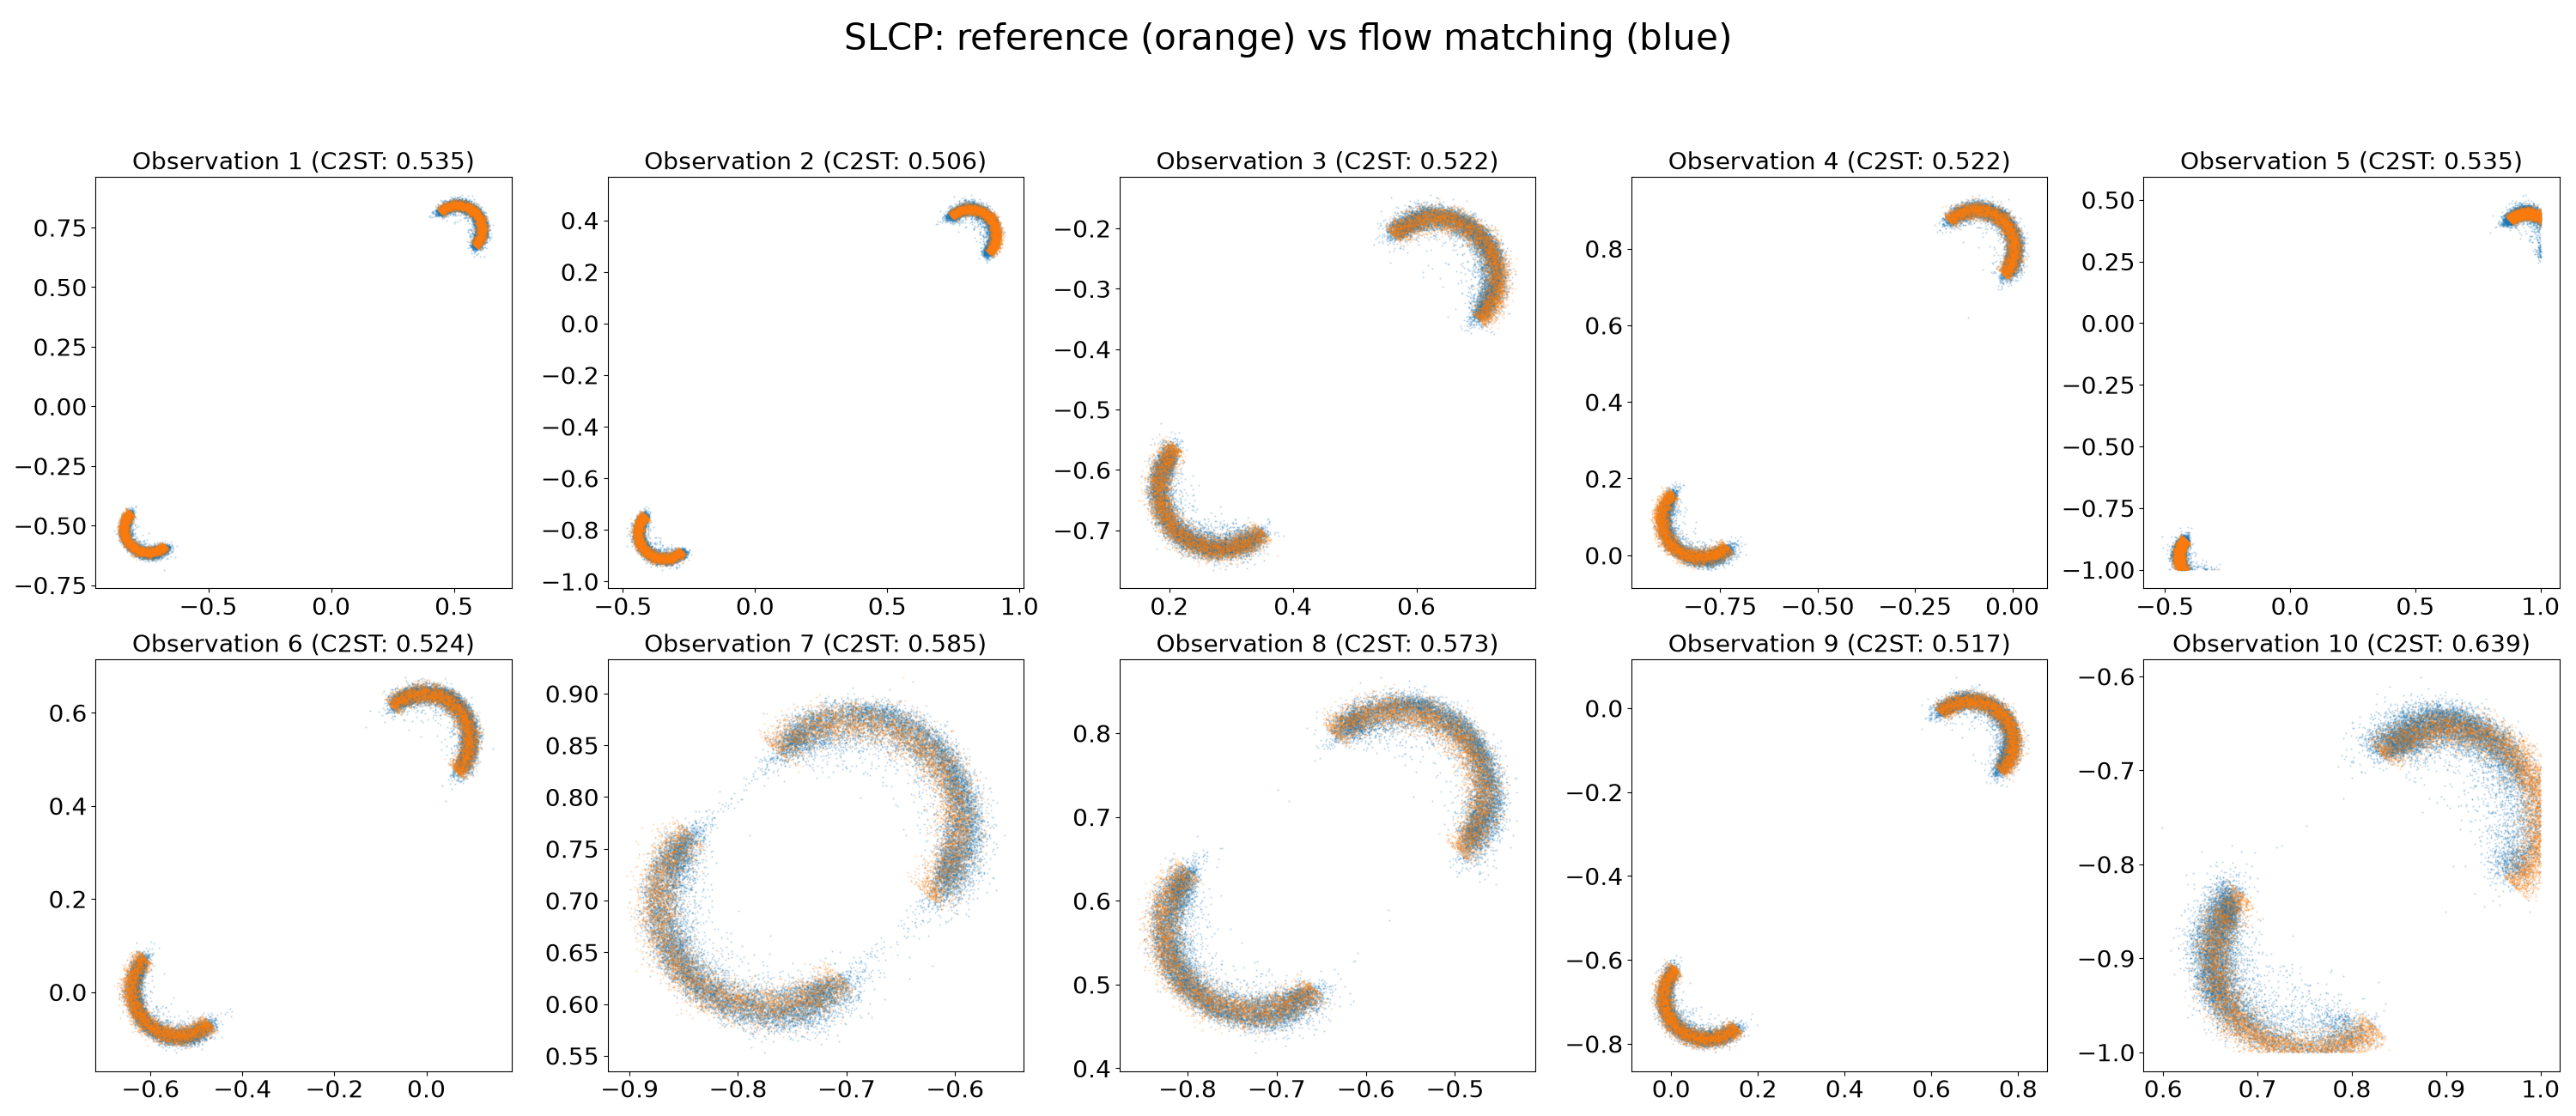
\includegraphics[width=0.9\textwidth]{posteriors_fmpe_two_moons.png}
	% TODO: drifting panel alongside
\end{frame}

\begin{frame}
	\frametitle{SLCP}
	\begin{columns}[c]
		\column{0.5\textwidth}
			\centering
			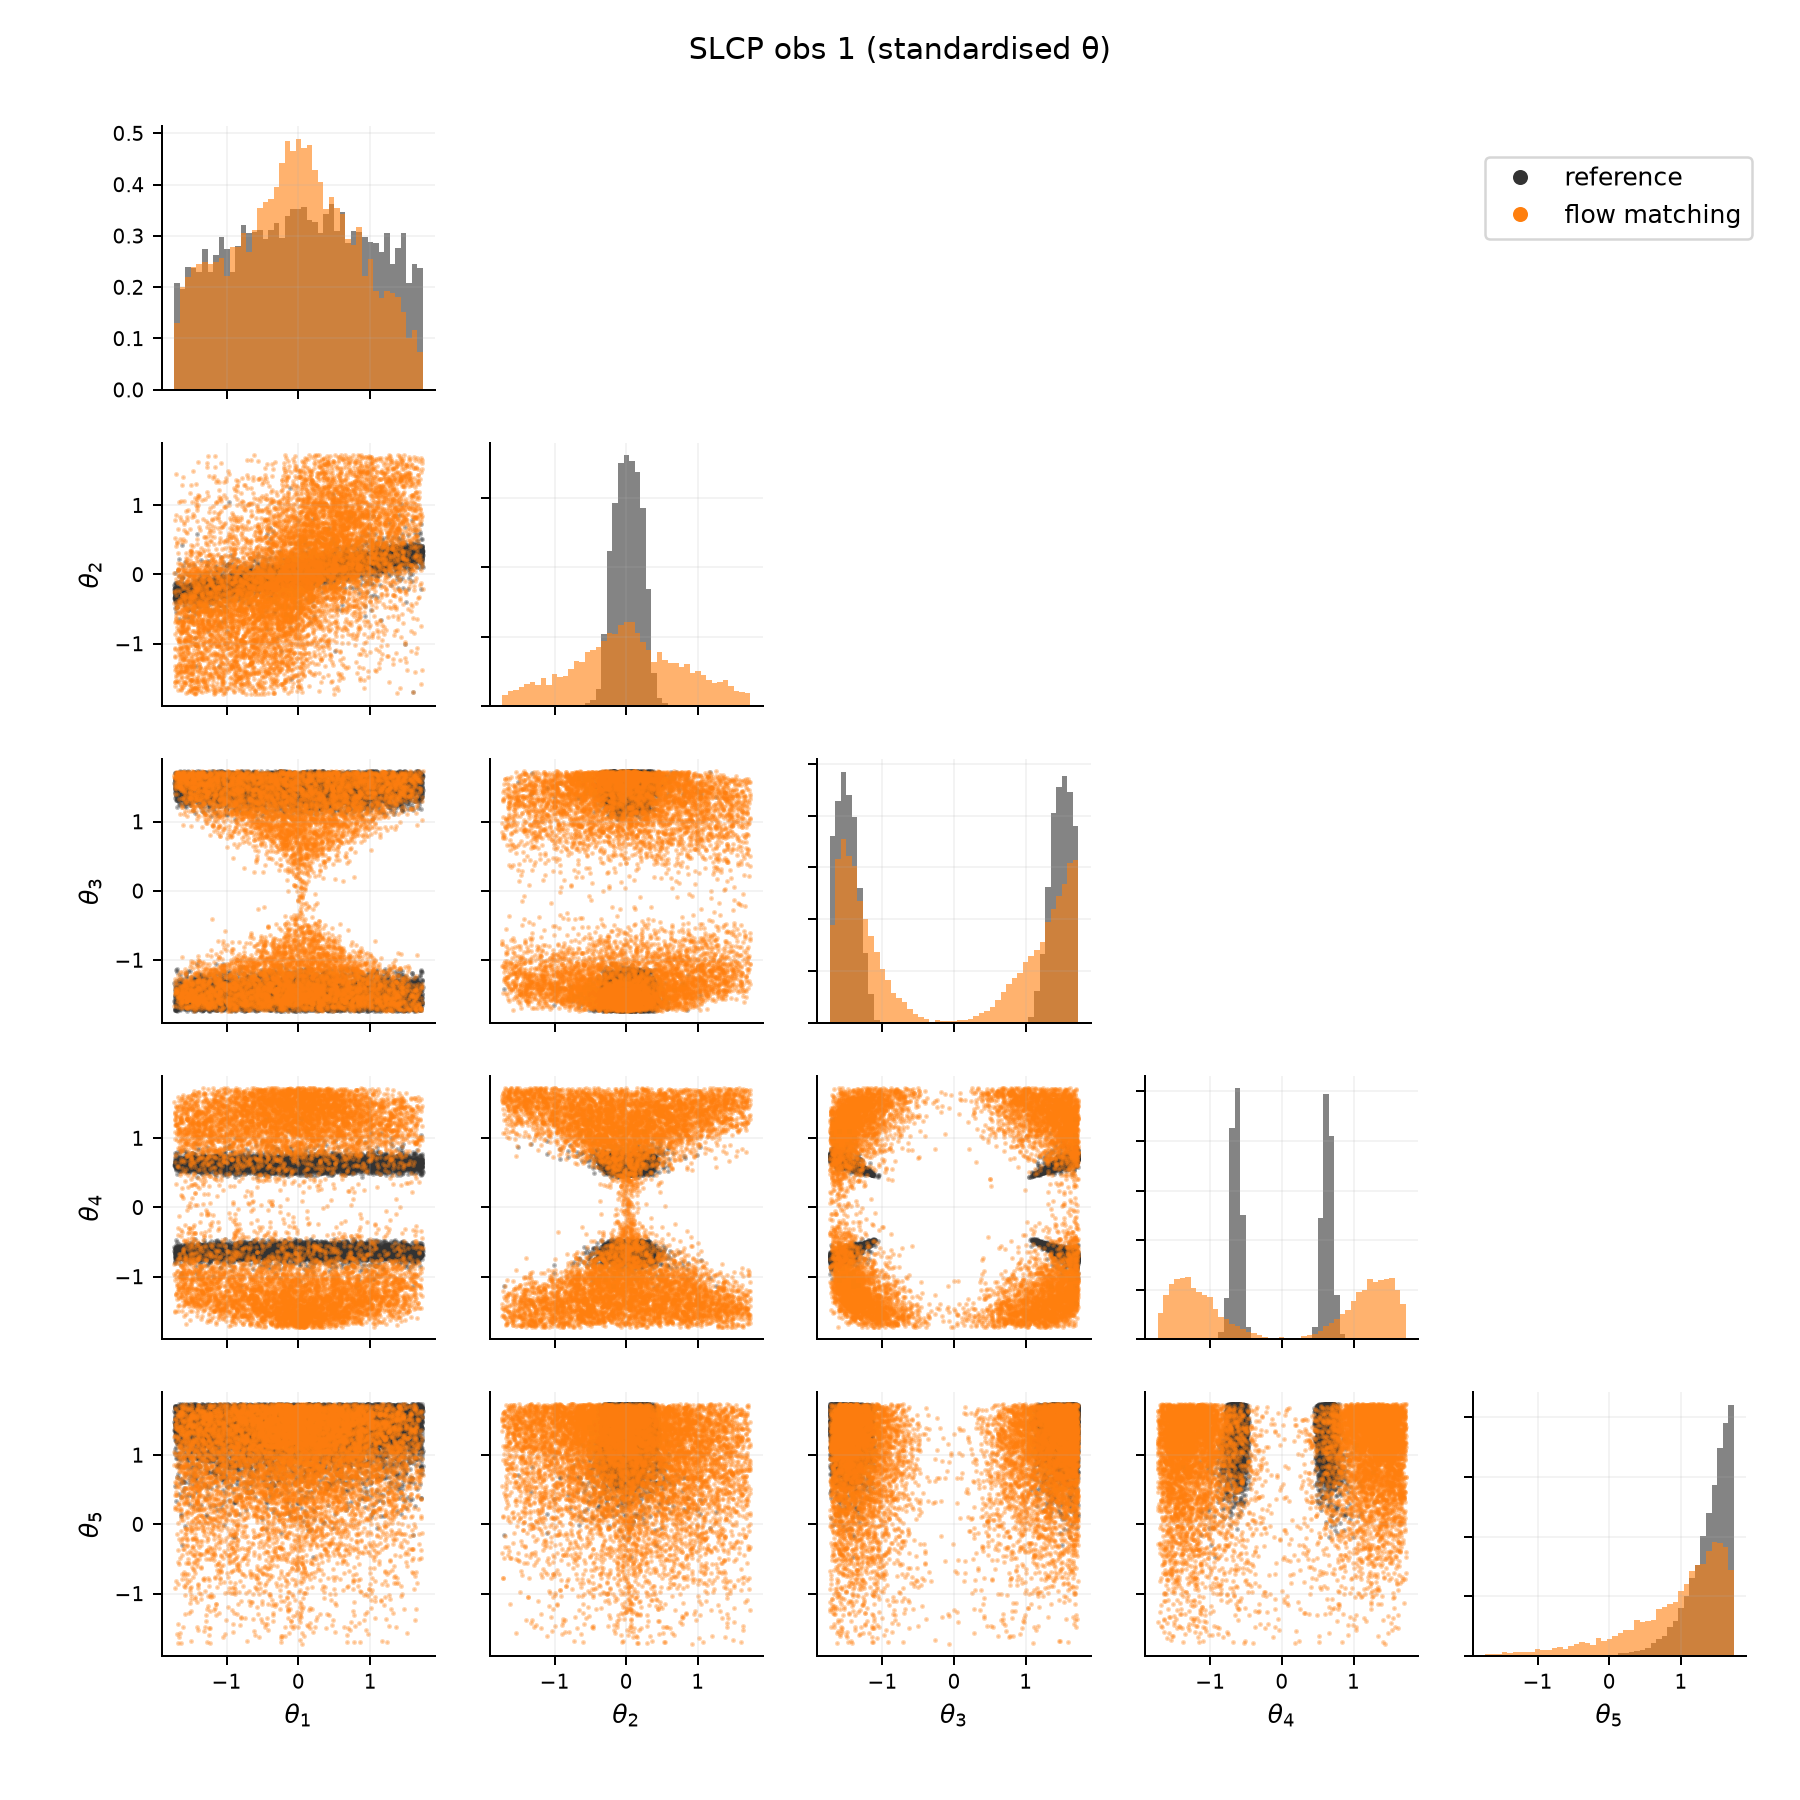
\includegraphics[width=\textwidth]{flow_matching_SLCP_marginals.png}

			\small Flow matching
		\column{0.5\textwidth}
			\centering
			\includegraphics[draft,width=\textwidth]{drifting_SLCP_marginals.png}

			\small Drifting
	\end{columns}
\end{frame}

\begin{frame}
	\frametitle{Lotka--Volterra}
	\begin{columns}[c]
		\column{0.5\textwidth}
			\centering
			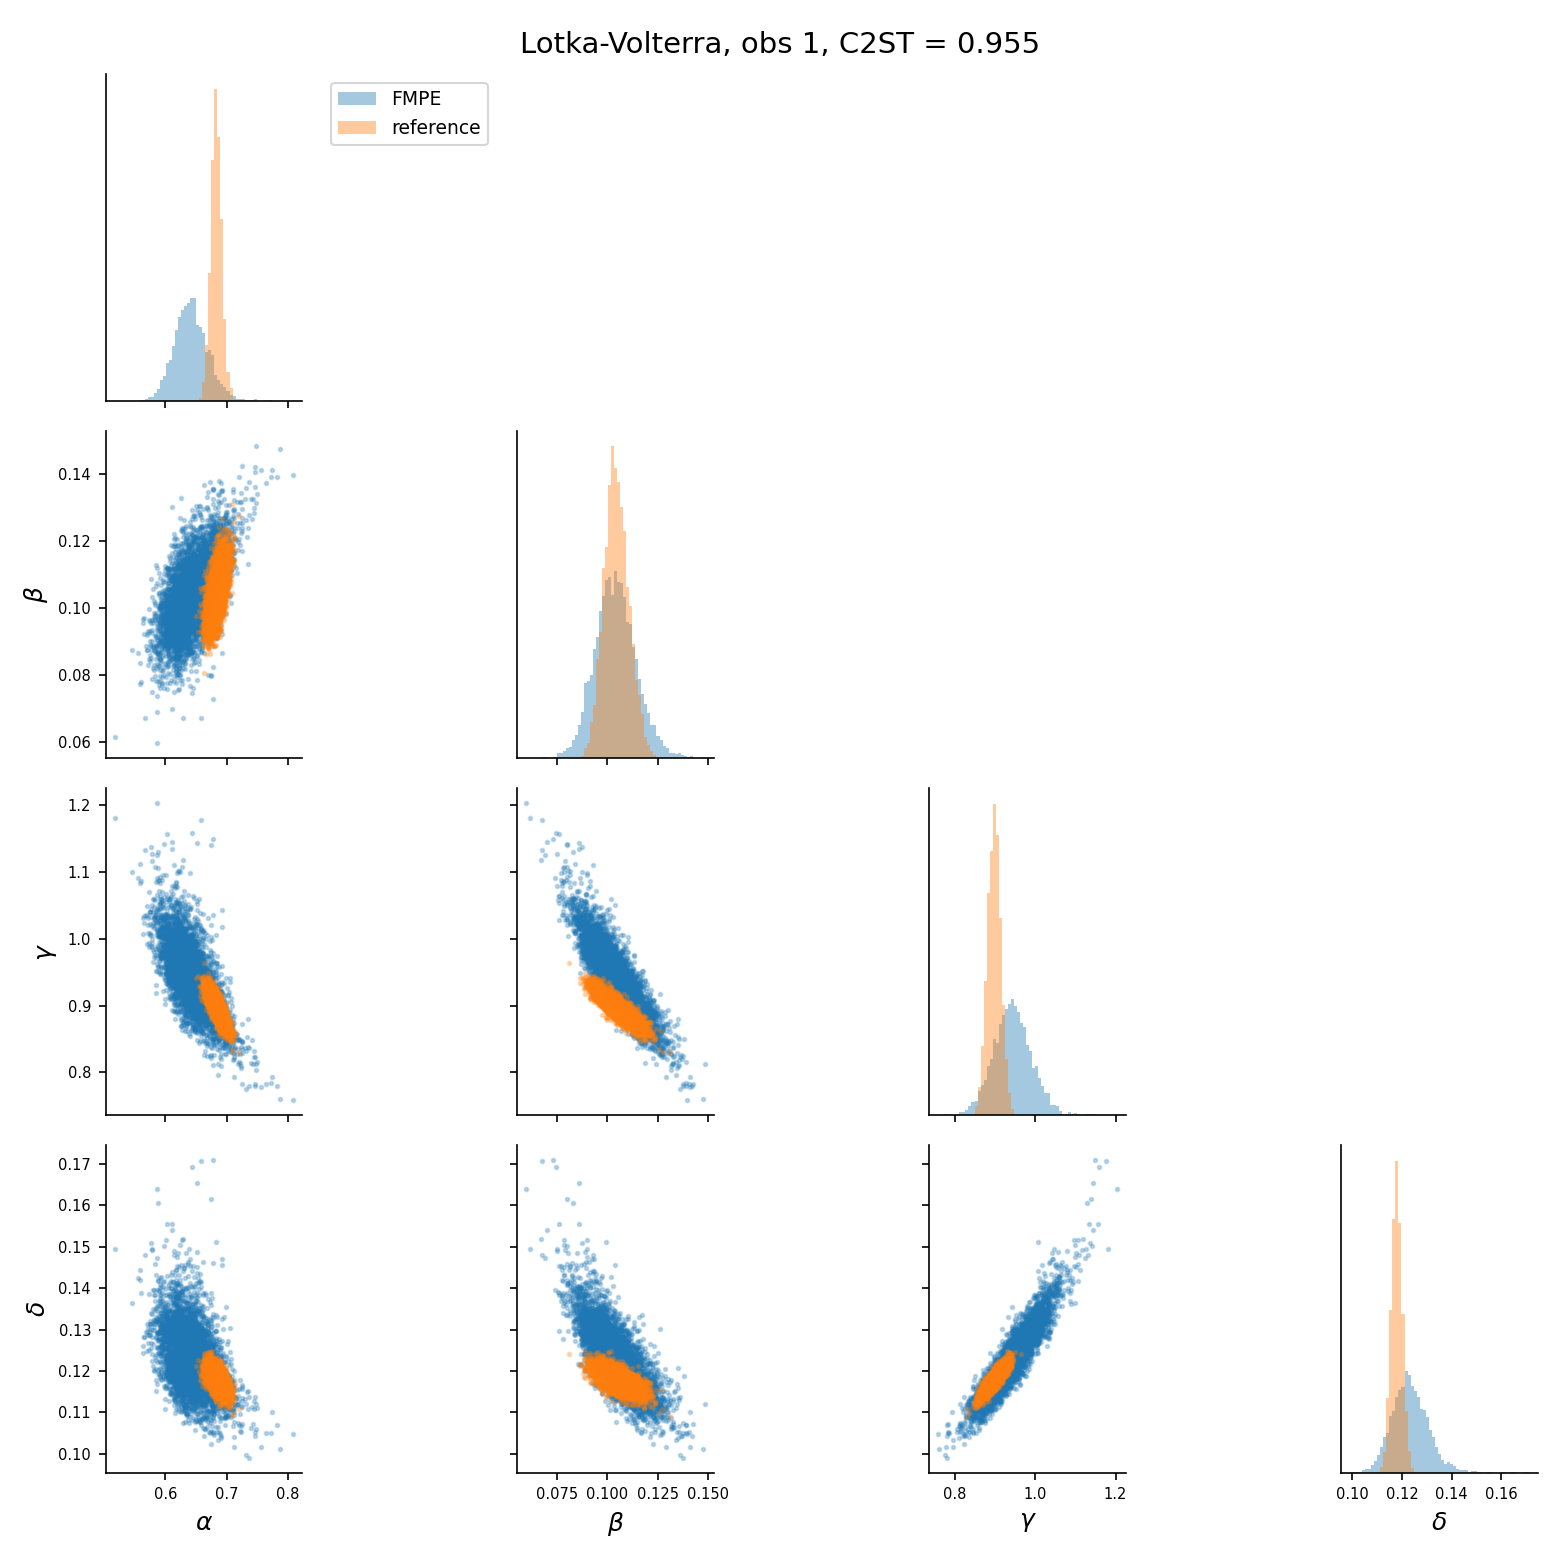
\includegraphics[width=\textwidth]{corner_obs1.png}

			\small FMPE, observation 1
		\column{0.5\textwidth}
			\centering
			\includegraphics[draft,width=\textwidth]{drifting_lv_predictive.png}

			\small Drifting, posterior predictive
	\end{columns}
\end{frame}

\begin{frame}
	\frametitle{Results summary}
	\begin{table}
		\centering
		\begin{tabular}{lcc}
			\toprule
			Task & FMPE C2ST & Drifting C2ST \\
			\midrule
			Two Moons      & -- & -- \\
			SLCP           & -- & -- \\
			Lotka--Volterra & -- & -- \\
			\midrule
			Network passes per sample & $\sim$250 & 1 \\
			\bottomrule
		\end{tabular}
	\end{table}
	% TODO: fill in mean C2ST over the 10 sbibm observations
\end{frame}


% =============================================================================
\section{Conclusions}

\begin{frame}
	\frametitle{Conclusions}
	\begin{itemize}
		\item Flow matching: accurate, mass-covering, exact density --- but many-step sampling
		\item Drifting: one-step sampling, fast posterior predictive checks
		\item Joint Drifting adapts drifting to SBI without conditional samples
		\item Next steps: same test observations and references for both methods, calibration (SBC)
	\end{itemize}
\end{frame}

\begin{frame}
	\centering
	\Large Thank you --- questions?
\end{frame}

\end{document}
